\chapter{Matchings}
\makeheading{2020-03-01}
\section{Matching}
Given a set $ S $ of students and a set $ J $ of co-op jobs, how many positions
can we fill given that
\begin{itemize}
    \item each student in $ S $ has some set of jobs they are willing to do, and
    \item each job in $ J $ has some set of students that can do it
\end{itemize}
We can model this situation with a graph (where the set of dotted lines is a possible matching)
\tikzset{every picture/.style={line width=0.75pt}} %set default line width to 0.75pt        
\begin{center}
    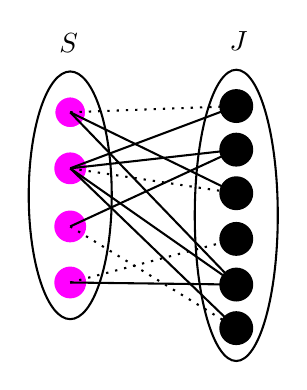
\begin{tikzpicture}[x=0.75pt,y=0.75pt,yscale=-1,xscale=1]
        %uncomment if require: \path (0,300); %set diagram left start at 0, and has height of 300

        %Shape: Circle [id:dp874602739477983] 
        \draw  [color={rgb, 255:red, 255; green, 255; blue, 255 }  ,draw opacity=1 ][fill={rgb, 255:red, 255; green, 0; blue, 255 }  ,fill opacity=1 ] (113,61.67) .. controls (113,57.43) and (116.43,54) .. (120.67,54) .. controls (124.9,54) and (128.33,57.43) .. (128.33,61.67) .. controls (128.33,65.9) and (124.9,69.33) .. (120.67,69.33) .. controls (116.43,69.33) and (113,65.9) .. (113,61.67) -- cycle ;
        %Shape: Circle [id:dp8073023708267365] 
        \draw  [draw opacity=0][fill={rgb, 255:red, 255; green, 0; blue, 255 }  ,fill opacity=1 ] (113,88.67) .. controls (113,84.43) and (116.43,81) .. (120.67,81) .. controls (124.9,81) and (128.33,84.43) .. (128.33,88.67) .. controls (128.33,92.9) and (124.9,96.33) .. (120.67,96.33) .. controls (116.43,96.33) and (113,92.9) .. (113,88.67) -- cycle ;
        %Shape: Circle [id:dp5011754824132996] 
        \draw  [draw opacity=0][fill={rgb, 255:red, 255; green, 0; blue, 255 }  ,fill opacity=1 ] (113,116.67) .. controls (113,112.43) and (116.43,109) .. (120.67,109) .. controls (124.9,109) and (128.33,112.43) .. (128.33,116.67) .. controls (128.33,120.9) and (124.9,124.33) .. (120.67,124.33) .. controls (116.43,124.33) and (113,120.9) .. (113,116.67) -- cycle ;
        %Shape: Circle [id:dp379883940516321] 
        \draw  [draw opacity=0][fill={rgb, 255:red, 255; green, 0; blue, 255 }  ,fill opacity=1 ] (113,143.67) .. controls (113,139.43) and (116.43,136) .. (120.67,136) .. controls (124.9,136) and (128.33,139.43) .. (128.33,143.67) .. controls (128.33,147.9) and (124.9,151.33) .. (120.67,151.33) .. controls (116.43,151.33) and (113,147.9) .. (113,143.67) -- cycle ;
        %Shape: Circle [id:dp7806171564733905] 
        \draw  [fill={rgb, 255:red, 0; green, 0; blue, 0 }  ,fill opacity=1 ] (193,58.67) .. controls (193,54.43) and (196.43,51) .. (200.67,51) .. controls (204.9,51) and (208.33,54.43) .. (208.33,58.67) .. controls (208.33,62.9) and (204.9,66.33) .. (200.67,66.33) .. controls (196.43,66.33) and (193,62.9) .. (193,58.67) -- cycle ;
        %Shape: Circle [id:dp5194402911666] 
        \draw  [fill={rgb, 255:red, 0; green, 0; blue, 0 }  ,fill opacity=1 ] (193,79.67) .. controls (193,75.43) and (196.43,72) .. (200.67,72) .. controls (204.9,72) and (208.33,75.43) .. (208.33,79.67) .. controls (208.33,83.9) and (204.9,87.33) .. (200.67,87.33) .. controls (196.43,87.33) and (193,83.9) .. (193,79.67) -- cycle ;
        %Shape: Circle [id:dp34062019757455597] 
        \draw  [fill={rgb, 255:red, 0; green, 0; blue, 0 }  ,fill opacity=1 ] (193,100.67) .. controls (193,96.43) and (196.43,93) .. (200.67,93) .. controls (204.9,93) and (208.33,96.43) .. (208.33,100.67) .. controls (208.33,104.9) and (204.9,108.33) .. (200.67,108.33) .. controls (196.43,108.33) and (193,104.9) .. (193,100.67) -- cycle ;
        %Shape: Circle [id:dp9595582437862881] 
        \draw  [fill={rgb, 255:red, 0; green, 0; blue, 0 }  ,fill opacity=1 ] (193,122.67) .. controls (193,118.43) and (196.43,115) .. (200.67,115) .. controls (204.9,115) and (208.33,118.43) .. (208.33,122.67) .. controls (208.33,126.9) and (204.9,130.33) .. (200.67,130.33) .. controls (196.43,130.33) and (193,126.9) .. (193,122.67) -- cycle ;
        %Shape: Circle [id:dp20156340027818953] 
        \draw  [fill={rgb, 255:red, 0; green, 0; blue, 0 }  ,fill opacity=1 ] (193,144.67) .. controls (193,140.43) and (196.43,137) .. (200.67,137) .. controls (204.9,137) and (208.33,140.43) .. (208.33,144.67) .. controls (208.33,148.9) and (204.9,152.33) .. (200.67,152.33) .. controls (196.43,152.33) and (193,148.9) .. (193,144.67) -- cycle ;
        %Shape: Ellipse [id:dp14445497901751425] 
        \draw   (120.67,42) .. controls (131.71,42) and (140.67,68.71) .. (140.67,101.67) .. controls (140.67,134.62) and (131.71,161.33) .. (120.67,161.33) .. controls (109.62,161.33) and (100.67,134.62) .. (100.67,101.67) .. controls (100.67,68.71) and (109.62,42) .. (120.67,42) -- cycle ;
        %Shape: Ellipse [id:dp25910260906438487] 
        \draw   (200.67,41.17) .. controls (211.71,41.17) and (220.67,72.58) .. (220.67,111.33) .. controls (220.67,150.09) and (211.71,181.5) .. (200.67,181.5) .. controls (189.62,181.5) and (180.67,150.09) .. (180.67,111.33) .. controls (180.67,72.58) and (189.62,41.17) .. (200.67,41.17) -- cycle ;
        %Straight Lines [id:da23901967463648377] 
        \draw  [dash pattern={on 0.84pt off 2.51pt}]  (120.67,61.67) -- (200.67,58.67) ;
        %Straight Lines [id:da7390967555353448] 
        \draw    (120.67,61.67) -- (169.87,85.65) -- (200.67,100.67) ;
        %Straight Lines [id:da23495347753003626] 
        \draw    (120.67,61.67) -- (200.67,144.67) ;
        %Shape: Circle [id:dp971087178505783] 
        \draw  [fill={rgb, 255:red, 0; green, 0; blue, 0 }  ,fill opacity=1 ] (193,165.67) .. controls (193,161.43) and (196.43,158) .. (200.67,158) .. controls (204.9,158) and (208.33,161.43) .. (208.33,165.67) .. controls (208.33,169.9) and (204.9,173.33) .. (200.67,173.33) .. controls (196.43,173.33) and (193,169.9) .. (193,165.67) -- cycle ;
        %Straight Lines [id:da18702222366927213] 
        \draw    (120.67,88.67) -- (200.67,79.67) ;
        %Straight Lines [id:da8547368268856821] 
        \draw    (120.67,88.67) -- (200.67,58.67) ;
        %Straight Lines [id:da866941551158453] 
        \draw  [dash pattern={on 0.84pt off 2.51pt}]  (120.67,88.67) -- (200.67,100.67) ;
        %Straight Lines [id:da19713460360165558] 
        \draw    (120.67,88.67) -- (200.67,144.67) ;
        %Straight Lines [id:da8482059266947752] 
        \draw    (120.67,88.67) -- (200.67,165.67) ;
        %Straight Lines [id:da761938782060283] 
        \draw    (120.67,116.67) -- (200.67,79.67) ;
        %Straight Lines [id:da6310586592176192] 
        \draw  [dash pattern={on 0.84pt off 2.51pt}]  (120.67,116.67) -- (200.67,165.67) ;
        %Straight Lines [id:da3481946467242253] 
        \draw  [dash pattern={on 0.84pt off 2.51pt}]  (120.67,143.67) -- (200.67,122.67) ;
        %Straight Lines [id:da012978277561190854] 
        \draw    (120.67,143.67) -- (200.67,144.67) ;

        % Text Node
        \draw (114,22.4) node [anchor=north west][inner sep=0.75pt]    {$S$};
        % Text Node
        \draw (196,21.4) node [anchor=north west][inner sep=0.75pt]    {$J$};
    \end{tikzpicture}

\end{center}
the vertices are $ S\cup J $, and we include an edge between student $ s $ and job $ j $
if and only if they are `compatible'.

\begin{defbox}
    \begin{definition}
        A \textbf{\emph{matching}} in a graph $ G $ is a set $ M $ of edges of $ G $
        so that no two edges in $ M $ have an end in common.
    \end{definition}
\end{defbox}
Asking for as many job assignments as possible is equivalent to asking for a largest
possible matching in the graph.

\begin{defbox}
    \begin{definition}
        Let $ G=(V,E) $ be a graph, and $ M $ be a matching of G
        \begin{itemize}
            \item A vertex $ v $ of $ G $ is \textbf{\emph{saturated}} by $ M $
                  if some edge in $ M $ has $ v $ as an end. Otherwise it is \textbf{\emph{unsaturated}}
                  (exposed). \underline{Note}: A matching of size $ k $ has $ 2k $ saturated vertices.
            \item $ M $ is a \textbf{\emph{maxim\underline{um} matching}} of $ G $ if $ G $ has no matching
                  larger than $ M $.
            \item $ M $ is a \textbf{\emph{maxim\underline{al} matching}} if $ M $ is contained in no larger
                  matching of $ G $. \underline{Note}: Maximum $ \implies $ Maximal, but the converse is not true.
        \end{itemize}

    \end{definition}
\end{defbox}

\tikzset{every picture/.style={line width=0.75pt}} %set default line width to 0.75pt       
\begin{figure}[!htbp]
    \centering
    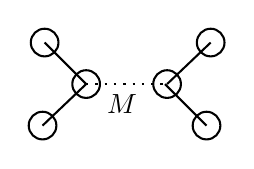
\begin{tikzpicture}[x=0.75pt,y=0.75pt,yscale=-1,xscale=1]
        %Shape: Circle [id:dp7068398656443018] 
        \draw   (115,119.67) .. controls (115,115.98) and (117.98,113) .. (121.67,113) .. controls (125.35,113) and (128.33,115.98) .. (128.33,119.67) .. controls (128.33,123.35) and (125.35,126.33) .. (121.67,126.33) .. controls (117.98,126.33) and (115,123.35) .. (115,119.67) -- cycle ;
        %Shape: Circle [id:dp6084217223946374] 
        \draw   (114,159.67) .. controls (114,155.98) and (116.98,153) .. (120.67,153) .. controls (124.35,153) and (127.33,155.98) .. (127.33,159.67) .. controls (127.33,163.35) and (124.35,166.33) .. (120.67,166.33) .. controls (116.98,166.33) and (114,163.35) .. (114,159.67) -- cycle ;
        %Shape: Circle [id:dp030307103377860245] 
        \draw   (135,139.67) .. controls (135,135.98) and (137.98,133) .. (141.67,133) .. controls (145.35,133) and (148.33,135.98) .. (148.33,139.67) .. controls (148.33,143.35) and (145.35,146.33) .. (141.67,146.33) .. controls (137.98,146.33) and (135,143.35) .. (135,139.67) -- cycle ;
        %Shape: Circle [id:dp34117637238791076] 
        \draw   (174,139.67) .. controls (174,135.98) and (176.98,133) .. (180.67,133) .. controls (184.35,133) and (187.33,135.98) .. (187.33,139.67) .. controls (187.33,143.35) and (184.35,146.33) .. (180.67,146.33) .. controls (176.98,146.33) and (174,143.35) .. (174,139.67) -- cycle ;
        %Shape: Circle [id:dp15014901482960308] 
        \draw   (195,119.67) .. controls (195,115.98) and (197.98,113) .. (201.67,113) .. controls (205.35,113) and (208.33,115.98) .. (208.33,119.67) .. controls (208.33,123.35) and (205.35,126.33) .. (201.67,126.33) .. controls (197.98,126.33) and (195,123.35) .. (195,119.67) -- cycle ;
        %Shape: Circle [id:dp9635762448621268] 
        \draw   (193,159.67) .. controls (193,155.98) and (195.98,153) .. (199.67,153) .. controls (203.35,153) and (206.33,155.98) .. (206.33,159.67) .. controls (206.33,163.35) and (203.35,166.33) .. (199.67,166.33) .. controls (195.98,166.33) and (193,163.35) .. (193,159.67) -- cycle ;
        %Straight Lines [id:da9749767456226316] 
        \draw    (121.67,119.67) -- (141.67,139.67) ;
        %Straight Lines [id:da30613474042529243] 
        \draw    (179.67,139.67) -- (199.67,159.67) ;
        %Straight Lines [id:da3243175396121116] 
        \draw    (120.67,159.67) -- (141.67,139.67) ;
        %Straight Lines [id:da9775132435040539] 
        \draw  [dash pattern={on 0.84pt off 2.51pt}]  (141.67,139.67) -- (179.67,139.67) ;
        %Straight Lines [id:da6894329645645343] 
        \draw    (180.67,139.67) -- (201.67,119.67) ;

        % Text Node
        \draw (150.33,143.07) node [anchor=north west][inner sep=0.75pt]    {$M$};
    \end{tikzpicture}
    \caption{Maximal, but not maximum matching.}
\end{figure}
\begin{defbox}
    \begin{definition}
        Let $ P $ be a path in a graph $ G=(V,E) $ and $ M $ be a mathcing of $ G $. Let
        $ e_1,e_2,\ldots ,e_k $ be the edges of $ P $ occurring in order. If $ M\cap E(P) $
        is either $ \{e_1,e_3,e_5,\ldots \} $ or $ \{e_2,e_4,e_6,\ldots\} $ then $ P $
        is an \textbf{\emph{$ \bm{M} $-alternating path}}. That is, the edges in $ P $
        alternate between being matching and non-matching edges. $ P $
        is an \textbf{\emph{$ \bm{M} $-augmenting path}} if $ M\cap E(P)=\{e_2,e_4,e_6,\ldots \} $,
        and also both ends of $ P $ are unsaturated vertices.
    \end{definition}
\end{defbox}
We can use an $ M $-augmenting path in a graph $ G $ to make a matching $ M^\prime $
of $ G $ that is larger than $ M $.

\begin{thmbox}
    \begin{prop}
        If $ M $ is a matching in $ G $ and $ P $ is an $ M $-augmenting path, then $ M $
        is not a maximum matching of $ G $.
    \end{prop}
\end{thmbox}
\begin{proof}
    Replace $ M $ with
    \[ \left( M\setminus (M\cap E(P)) \right)\cup (E(P)\setminus M) \]
    to get a larger matching than $ M $.
\end{proof}

\begin{figure}[!htbp]
    \centering
    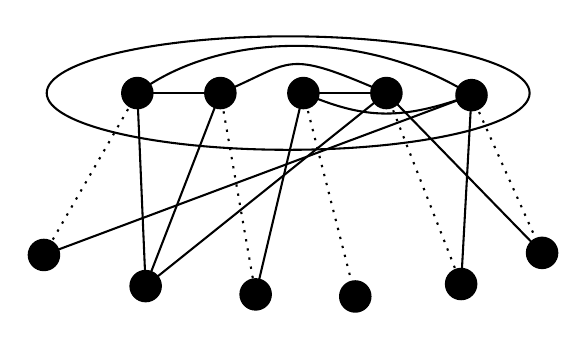
\begin{tikzpicture}[x=0.75pt,y=0.75pt,yscale=-1,xscale=1]
        %Shape: Circle [id:dp28394531065328943] 
        \draw  [color={rgb, 255:red, 0; green, 0; blue, 0 }  ,draw opacity=1 ][fill={rgb, 255:red, 0; green, 0; blue, 0 }  ,fill opacity=1 ] (193,39.33) .. controls (193,35.28) and (196.28,32) .. (200.33,32) .. controls (204.38,32) and (207.67,35.28) .. (207.67,39.33) .. controls (207.67,43.38) and (204.38,46.67) .. (200.33,46.67) .. controls (196.28,46.67) and (193,43.38) .. (193,39.33) -- cycle ;
        %Shape: Circle [id:dp906604373413785] 
        \draw  [fill={rgb, 255:red, 0; green, 0; blue, 0 }  ,fill opacity=1 ] (233,39.33) .. controls (233,35.28) and (236.28,32) .. (240.33,32) .. controls (244.38,32) and (247.67,35.28) .. (247.67,39.33) .. controls (247.67,43.38) and (244.38,46.67) .. (240.33,46.67) .. controls (236.28,46.67) and (233,43.38) .. (233,39.33) -- cycle ;
        %Shape: Circle [id:dp5708196148510684] 
        \draw  [fill={rgb, 255:red, 0; green, 0; blue, 0 }  ,fill opacity=1 ] (273,39.33) .. controls (273,35.28) and (276.28,32) .. (280.33,32) .. controls (284.38,32) and (287.67,35.28) .. (287.67,39.33) .. controls (287.67,43.38) and (284.38,46.67) .. (280.33,46.67) .. controls (276.28,46.67) and (273,43.38) .. (273,39.33) -- cycle ;
        %Shape: Circle [id:dp1238720705954427] 
        \draw  [fill={rgb, 255:red, 0; green, 0; blue, 0 }  ,fill opacity=1 ] (313,39.33) .. controls (313,35.28) and (316.28,32) .. (320.33,32) .. controls (324.38,32) and (327.67,35.28) .. (327.67,39.33) .. controls (327.67,43.38) and (324.38,46.67) .. (320.33,46.67) .. controls (316.28,46.67) and (313,43.38) .. (313,39.33) -- cycle ;
        %Shape: Circle [id:dp9292635440690116] 
        \draw  [fill={rgb, 255:red, 0; green, 0; blue, 0 }  ,fill opacity=1 ] (354,40.33) .. controls (354,36.28) and (357.28,33) .. (361.33,33) .. controls (365.38,33) and (368.67,36.28) .. (368.67,40.33) .. controls (368.67,44.38) and (365.38,47.67) .. (361.33,47.67) .. controls (357.28,47.67) and (354,44.38) .. (354,40.33) -- cycle ;
        %Shape: Ellipse [id:dp7742223337496057] 
        \draw   (156.67,39.33) .. controls (156.67,24.24) and (208.75,12) .. (273,12) .. controls (337.25,12) and (389.33,24.24) .. (389.33,39.33) .. controls (389.33,54.43) and (337.25,66.67) .. (273,66.67) .. controls (208.75,66.67) and (156.67,54.43) .. (156.67,39.33) -- cycle ;
        %Straight Lines [id:da5982639993522213] 
        \draw    (200.33,39.33) -- (240.33,39.33) ;
        %Straight Lines [id:da4026846985847934] 
        \draw    (280.33,39.33) -- (320.33,39.33) ;
        %Curve Lines [id:da004621287127507645] 
        \draw    (200.33,39.33) .. controls (240.33,9.33) and (310.67,8.33) .. (361.33,40.33) ;
        %Curve Lines [id:da6408000655186094] 
        \draw    (280.33,39.33) .. controls (310.67,52.33) and (327.67,52.33) .. (361.33,40.33) ;
        %Curve Lines [id:da8107526215021639] 
        \draw    (240.33,39.33) .. controls (276.67,24.33) and (269.67,17.33) .. (320.33,39.33) ;
        %Shape: Circle [id:dp7536735312594758] 
        \draw  [color={rgb, 255:red, 0; green, 0; blue, 0 }  ,draw opacity=1 ][fill={rgb, 255:red, 0; green, 0; blue, 0 }  ,fill opacity=1 ] (148,117.33) .. controls (148,113.28) and (151.28,110) .. (155.33,110) .. controls (159.38,110) and (162.67,113.28) .. (162.67,117.33) .. controls (162.67,121.38) and (159.38,124.67) .. (155.33,124.67) .. controls (151.28,124.67) and (148,121.38) .. (148,117.33) -- cycle ;
        %Shape: Circle [id:dp4958591543042232] 
        \draw  [color={rgb, 255:red, 0; green, 0; blue, 0 }  ,draw opacity=1 ][fill={rgb, 255:red, 0; green, 0; blue, 0 }  ,fill opacity=1 ] (197,132.33) .. controls (197,128.28) and (200.28,125) .. (204.33,125) .. controls (208.38,125) and (211.67,128.28) .. (211.67,132.33) .. controls (211.67,136.38) and (208.38,139.67) .. (204.33,139.67) .. controls (200.28,139.67) and (197,136.38) .. (197,132.33) -- cycle ;
        %Shape: Circle [id:dp9030290836628191] 
        \draw  [color={rgb, 255:red, 0; green, 0; blue, 0 }  ,draw opacity=1 ][fill={rgb, 255:red, 0; green, 0; blue, 0 }  ,fill opacity=1 ] (250,136.33) .. controls (250,132.28) and (253.28,129) .. (257.33,129) .. controls (261.38,129) and (264.67,132.28) .. (264.67,136.33) .. controls (264.67,140.38) and (261.38,143.67) .. (257.33,143.67) .. controls (253.28,143.67) and (250,140.38) .. (250,136.33) -- cycle ;
        %Shape: Circle [id:dp16066689024693437] 
        \draw  [color={rgb, 255:red, 0; green, 0; blue, 0 }  ,draw opacity=1 ][fill={rgb, 255:red, 0; green, 0; blue, 0 }  ,fill opacity=1 ] (298,137.33) .. controls (298,133.28) and (301.28,130) .. (305.33,130) .. controls (309.38,130) and (312.67,133.28) .. (312.67,137.33) .. controls (312.67,141.38) and (309.38,144.67) .. (305.33,144.67) .. controls (301.28,144.67) and (298,141.38) .. (298,137.33) -- cycle ;
        %Shape: Circle [id:dp16091308830394613] 
        \draw  [color={rgb, 255:red, 0; green, 0; blue, 0 }  ,draw opacity=1 ][fill={rgb, 255:red, 0; green, 0; blue, 0 }  ,fill opacity=1 ] (349,131.33) .. controls (349,127.28) and (352.28,124) .. (356.33,124) .. controls (360.38,124) and (363.67,127.28) .. (363.67,131.33) .. controls (363.67,135.38) and (360.38,138.67) .. (356.33,138.67) .. controls (352.28,138.67) and (349,135.38) .. (349,131.33) -- cycle ;
        %Shape: Circle [id:dp6961709101648996] 
        \draw  [color={rgb, 255:red, 0; green, 0; blue, 0 }  ,draw opacity=1 ][fill={rgb, 255:red, 0; green, 0; blue, 0 }  ,fill opacity=1 ] (388,116.33) .. controls (388,112.28) and (391.28,109) .. (395.33,109) .. controls (399.38,109) and (402.67,112.28) .. (402.67,116.33) .. controls (402.67,120.38) and (399.38,123.67) .. (395.33,123.67) .. controls (391.28,123.67) and (388,120.38) .. (388,116.33) -- cycle ;
        %Straight Lines [id:da6896069134113437] 
        \draw  [dash pattern={on 0.84pt off 2.51pt}]  (200.33,39.33) -- (155.33,117.33) ;
        %Straight Lines [id:da5374603598481258] 
        \draw    (200.33,39.33) -- (204.33,132.33) ;
        %Straight Lines [id:da692007056075935] 
        \draw    (240.33,39.33) -- (204.33,132.33) ;
        %Straight Lines [id:da5014721599881928] 
        \draw  [dash pattern={on 0.84pt off 2.51pt}]  (240.33,39.33) -- (257.33,136.33) ;
        %Straight Lines [id:da6520996475913642] 
        \draw    (280.33,39.33) -- (257.33,136.33) ;
        %Straight Lines [id:da7518580596524546] 
        \draw  [dash pattern={on 0.84pt off 2.51pt}]  (280.33,39.33) -- (305.33,137.33) ;
        %Straight Lines [id:da8737611139996777] 
        \draw    (320.33,39.33) -- (204.33,132.33) ;
        %Straight Lines [id:da14946780575048801] 
        \draw  [dash pattern={on 0.84pt off 2.51pt}]  (320.33,39.33) -- (356.33,131.33) ;
        %Straight Lines [id:da23692569021756804] 
        \draw    (320.33,39.33) -- (395.33,116.33) ;
        %Straight Lines [id:da12684548331456647] 
        \draw    (361.33,40.33) -- (155.33,117.33) ;
        %Straight Lines [id:da728991854059622] 
        \draw    (361.33,40.33) -- (356.33,131.33) ;
        %Straight Lines [id:da5603840111269398] 
        \draw  [dash pattern={on 0.84pt off 2.51pt}]  (361.33,40.33) -- (395.33,116.33) ;

    \end{tikzpicture}
    \caption{Vertex Cover}
\end{figure}
Clearly, it is not possible to have a matching of size $ 6 $ here.
The matching above covers all edges of the graph.
\begin{defbox}
    \begin{definition}
        A (vertex) \textbf{\emph{cover}} of a graph $ G $ is a set $ C\subseteq V(G) $ such that
        every edge of $ G $ has at least one end in $ C $.
    \end{definition}
\end{defbox}

\begin{thmbox}
    \begin{prop}\label{cover prop}
        If $ C $ is a cover of $ G $ and $ M $ is a matching of $ G $, then
        \[ |M|\leqslant |C| \]
    \end{prop}
\end{thmbox}
\begin{proof}
    We use the pigeonhole principle. Each edge in $ M $ has an end in $ C $ by the definition
    of a cover. Since $ M $ is a matching, these ends are distinct. So
    \[ |C|\geqslant |M| \]
\end{proof}

\begin{thmbox}
    \begin{prop}
        If $ C $ is a cover of $ G $ and $ M $ is a matching of $ G $ with $ |M|=|C| $,
        then $ M $ is a maximum matching of $ G $, and $ C $ is a minimum (smallest possible)
        cover of $ G $.
    \end{prop}
\end{thmbox}
\begin{proof}
    Let $ M_0 $ be a maximum matching, and $ C_0 $ be a minimum cover. Then,
    \begin{equation}
        \begin{aligned}
            |M| & \leqslant |M_0| & M_0\text{ is a maximum matching} \\
                & \leqslant |C_0| & \text{by \ref{cover prop}}       \\
                & \leqslant |C|   & C_0 \text{ is a minimum cover}   \\
                & =|M|            & \text{by assumption}
        \end{aligned}
    \end{equation}
    Equality holds throughout, so $ |M|=|M_0| $, which means that $ M $ is a maximum
    matching and $ |C|=|C_0| $ means that $ C $ is a minimum cover.
\end{proof}
$ \dagger $\underline{Note}: Usually, $ \nu(G) = $ size of a maximum matching of $ G $,
and $ \tau(G) = $ size of a minimum cover of $ G $.

\ref{cover prop} states that, for any $ G $,
\[ |\text{maximum matching of }G|\leqslant |\text{minimum cover of }G| \]
\begin{center}
    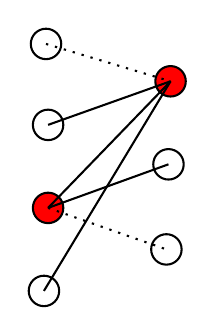
\begin{tikzpicture}[x=0.75pt,y=0.75pt,yscale=-1,xscale=1]
        %uncomment if require: \path (0,300); %set diagram left start at 0, and has height of 300

        %Shape: Circle [id:dp37545667714417985] 
        \draw   (153,80.33) .. controls (153,76.28) and (156.28,73) .. (160.33,73) .. controls (164.38,73) and (167.67,76.28) .. (167.67,80.33) .. controls (167.67,84.38) and (164.38,87.67) .. (160.33,87.67) .. controls (156.28,87.67) and (153,84.38) .. (153,80.33) -- cycle ;
        %Shape: Circle [id:dp027414498179569313] 
        \draw   (154,119.33) .. controls (154,115.28) and (157.28,112) .. (161.33,112) .. controls (165.38,112) and (168.67,115.28) .. (168.67,119.33) .. controls (168.67,123.38) and (165.38,126.67) .. (161.33,126.67) .. controls (157.28,126.67) and (154,123.38) .. (154,119.33) -- cycle ;
        %Shape: Circle [id:dp1814994392561211] 
        \draw  [fill={rgb, 255:red, 255; green, 0; blue, 0 }  ,fill opacity=1 ] (154,159.33) .. controls (154,155.28) and (157.28,152) .. (161.33,152) .. controls (165.38,152) and (168.67,155.28) .. (168.67,159.33) .. controls (168.67,163.38) and (165.38,166.67) .. (161.33,166.67) .. controls (157.28,166.67) and (154,163.38) .. (154,159.33) -- cycle ;
        %Shape: Circle [id:dp7478691255246693] 
        \draw   (152,199.33) .. controls (152,195.28) and (155.28,192) .. (159.33,192) .. controls (163.38,192) and (166.67,195.28) .. (166.67,199.33) .. controls (166.67,203.38) and (163.38,206.67) .. (159.33,206.67) .. controls (155.28,206.67) and (152,203.38) .. (152,199.33) -- cycle ;
        %Shape: Circle [id:dp9725895928459528] 
        \draw  [fill={rgb, 255:red, 255; green, 0; blue, 0 }  ,fill opacity=1 ] (213,98.33) .. controls (213,94.28) and (216.28,91) .. (220.33,91) .. controls (224.38,91) and (227.67,94.28) .. (227.67,98.33) .. controls (227.67,102.38) and (224.38,105.67) .. (220.33,105.67) .. controls (216.28,105.67) and (213,102.38) .. (213,98.33) -- cycle ;
        %Shape: Circle [id:dp018874034924878935] 
        \draw   (212,138.33) .. controls (212,134.28) and (215.28,131) .. (219.33,131) .. controls (223.38,131) and (226.67,134.28) .. (226.67,138.33) .. controls (226.67,142.38) and (223.38,145.67) .. (219.33,145.67) .. controls (215.28,145.67) and (212,142.38) .. (212,138.33) -- cycle ;
        %Shape: Circle [id:dp428348938541543] 
        \draw   (211,179.33) .. controls (211,175.28) and (214.28,172) .. (218.33,172) .. controls (222.38,172) and (225.67,175.28) .. (225.67,179.33) .. controls (225.67,183.38) and (222.38,186.67) .. (218.33,186.67) .. controls (214.28,186.67) and (211,183.38) .. (211,179.33) -- cycle ;
        %Straight Lines [id:da3798612178271693] 
        \draw  [dash pattern={on 0.84pt off 2.51pt}]  (160.33,80.33) -- (220.33,98.33) ;
        %Straight Lines [id:da9981436985819622] 
        \draw    (161.33,119.33) -- (220.33,98.33) ;
        %Straight Lines [id:da9978742344804361] 
        \draw    (161.33,159.33) -- (220.33,98.33) ;
        %Straight Lines [id:da34447893856426004] 
        \draw    (159.33,199.33) -- (220.33,98.33) ;
        %Straight Lines [id:da11811238473631136] 
        \draw    (161.33,159.33) -- (219.33,138.33) ;
        %Straight Lines [id:da09037290795458763] 
        \draw  [dash pattern={on 0.84pt off 2.51pt}]  (161.33,159.33) -- (218.33,179.33) ;

    \end{tikzpicture}

\end{center}
Deleting the red vertices $ \implies |C|= 2 $.
\[ |\text{maximum matching of G}| = 2 = |\text{minimum cover of } G| \]
However, this is not always true as seen below.
\begin{center}


    \tikzset{every picture/.style={line width=0.75pt}} %set default line width to 0.75pt        

    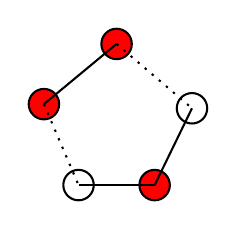
\begin{tikzpicture}[x=0.75pt,y=0.75pt,yscale=-1,xscale=1]
        %uncomment if require: \path (0,300); %set diagram left start at 0, and has height of 300

        %Shape: Circle [id:dp21271731455319154] 
        \draw  [fill={rgb, 255:red, 255; green, 0; blue, 0 }  ,fill opacity=1 ] (153,80.33) .. controls (153,76.28) and (156.28,73) .. (160.33,73) .. controls (164.38,73) and (167.67,76.28) .. (167.67,80.33) .. controls (167.67,84.38) and (164.38,87.67) .. (160.33,87.67) .. controls (156.28,87.67) and (153,84.38) .. (153,80.33) -- cycle ;
        %Straight Lines [id:da3377214309921256] 
        \draw  [dash pattern={on 0.84pt off 2.51pt}]  (160.33,80.33) -- (196.67,111.33) ;
        %Shape: Circle [id:dp15239788247965558] 
        \draw   (189.33,111.33) .. controls (189.33,107.28) and (192.62,104) .. (196.67,104) .. controls (200.72,104) and (204,107.28) .. (204,111.33) .. controls (204,115.38) and (200.72,118.67) .. (196.67,118.67) .. controls (192.62,118.67) and (189.33,115.38) .. (189.33,111.33) -- cycle ;
        %Shape: Circle [id:dp23851318758307316] 
        \draw  [fill={rgb, 255:red, 255; green, 0; blue, 0 }  ,fill opacity=1 ] (171.33,148.33) .. controls (171.33,144.28) and (174.62,141) .. (178.67,141) .. controls (182.72,141) and (186,144.28) .. (186,148.33) .. controls (186,152.38) and (182.72,155.67) .. (178.67,155.67) .. controls (174.62,155.67) and (171.33,152.38) .. (171.33,148.33) -- cycle ;
        %Shape: Circle [id:dp7542134009048679] 
        \draw   (134.67,148.33) .. controls (134.67,144.28) and (137.95,141) .. (142,141) .. controls (146.05,141) and (149.33,144.28) .. (149.33,148.33) .. controls (149.33,152.38) and (146.05,155.67) .. (142,155.67) .. controls (137.95,155.67) and (134.67,152.38) .. (134.67,148.33) -- cycle ;
        %Shape: Circle [id:dp2905682972946412] 
        \draw  [fill={rgb, 255:red, 255; green, 0; blue, 0 }  ,fill opacity=1 ] (118,109.33) .. controls (118,105.28) and (121.28,102) .. (125.33,102) .. controls (129.38,102) and (132.67,105.28) .. (132.67,109.33) .. controls (132.67,113.38) and (129.38,116.67) .. (125.33,116.67) .. controls (121.28,116.67) and (118,113.38) .. (118,109.33) -- cycle ;
        %Straight Lines [id:da5951249649317308] 
        \draw  [dash pattern={on 0.84pt off 2.51pt}]  (125.33,109.33) -- (142,148.33) ;
        %Straight Lines [id:da9315783025334317] 
        \draw    (160.33,80.33) -- (125.33,109.33) ;
        %Straight Lines [id:da5654511839083125] 
        \draw    (196.67,111.33) -- (178.67,148.33) ;
        %Straight Lines [id:da11049229477166267] 
        \draw    (178.67,148.33) -- (142,148.33) ;

    \end{tikzpicture}

\end{center}
\[ |\text{maximum matching of G}| = 2 \neq 3= |\text{minimum cover of } G| \]
